\uuid{eo6K}
\exo7id{5008}
\titre{exo7 5008}
\auteur{quercia}
\organisation{exo7}
\datecreate{2010-03-17}
\isIndication{false}
\isCorrection{true}
\chapitre{Courbes planes}
\sousChapitre{Points de rebroussement}
\module{Géométrie}
\niveau{L2}
\difficulte{}

\contenu{
\texte{

}
\begin{enumerate}
    \item \question{$x=2t^3+3t^2$, $y=3t^2+6t$                  

% 
% %-----------------------------------------------------------------------------
% \vtop to 7cm{\mapleplot{% img25
% x:=2*t^3+3*t^2;
% y:=3*t^2+6*t;
% print(plot([x,y,t=-3..3],-6..4,-3..3));}  \par
% \vss}}
\reponse{$$
\centerline{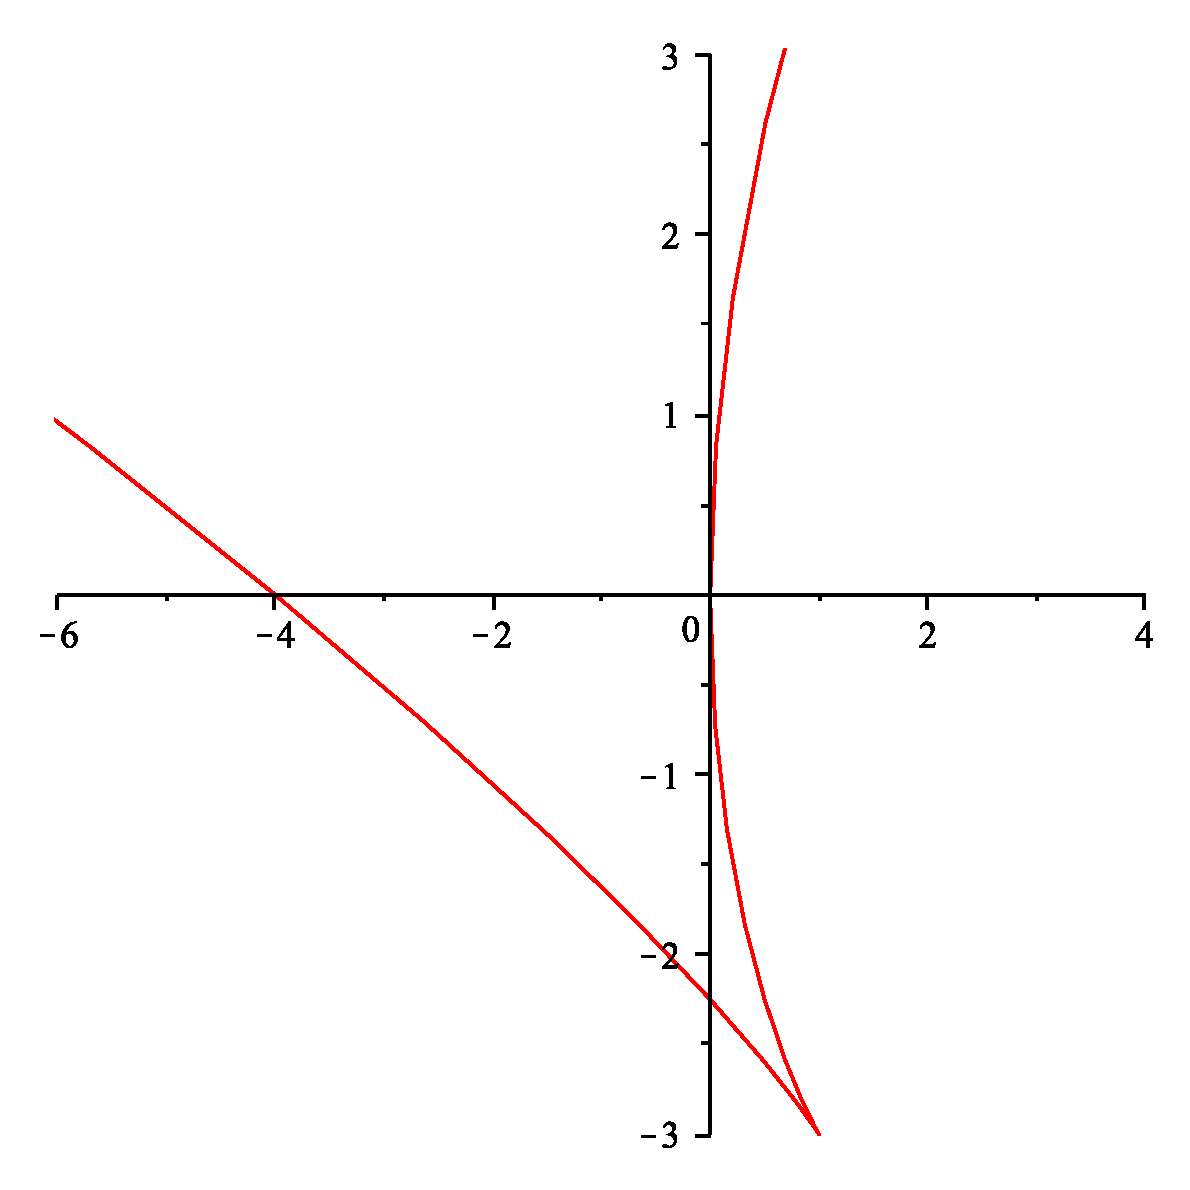
\includegraphics[height=4cm]{../images/img005008-1}}
$$
branche parabolique horizontale}
    \item \question{$x=t^3-3t$, $y=t^3-t^2-t+1$ 
% %-----------------------------------------------------------------------------
% \vtop to 7cm{\mapleplot{% img26
% x:=t^3-3*t;
% y:=t^3-t^2-t+1;
% print(plot([x,y,t=-3..3],-10..10,-7..7));}   \par
% \vss}}
\reponse{$$
\centerline{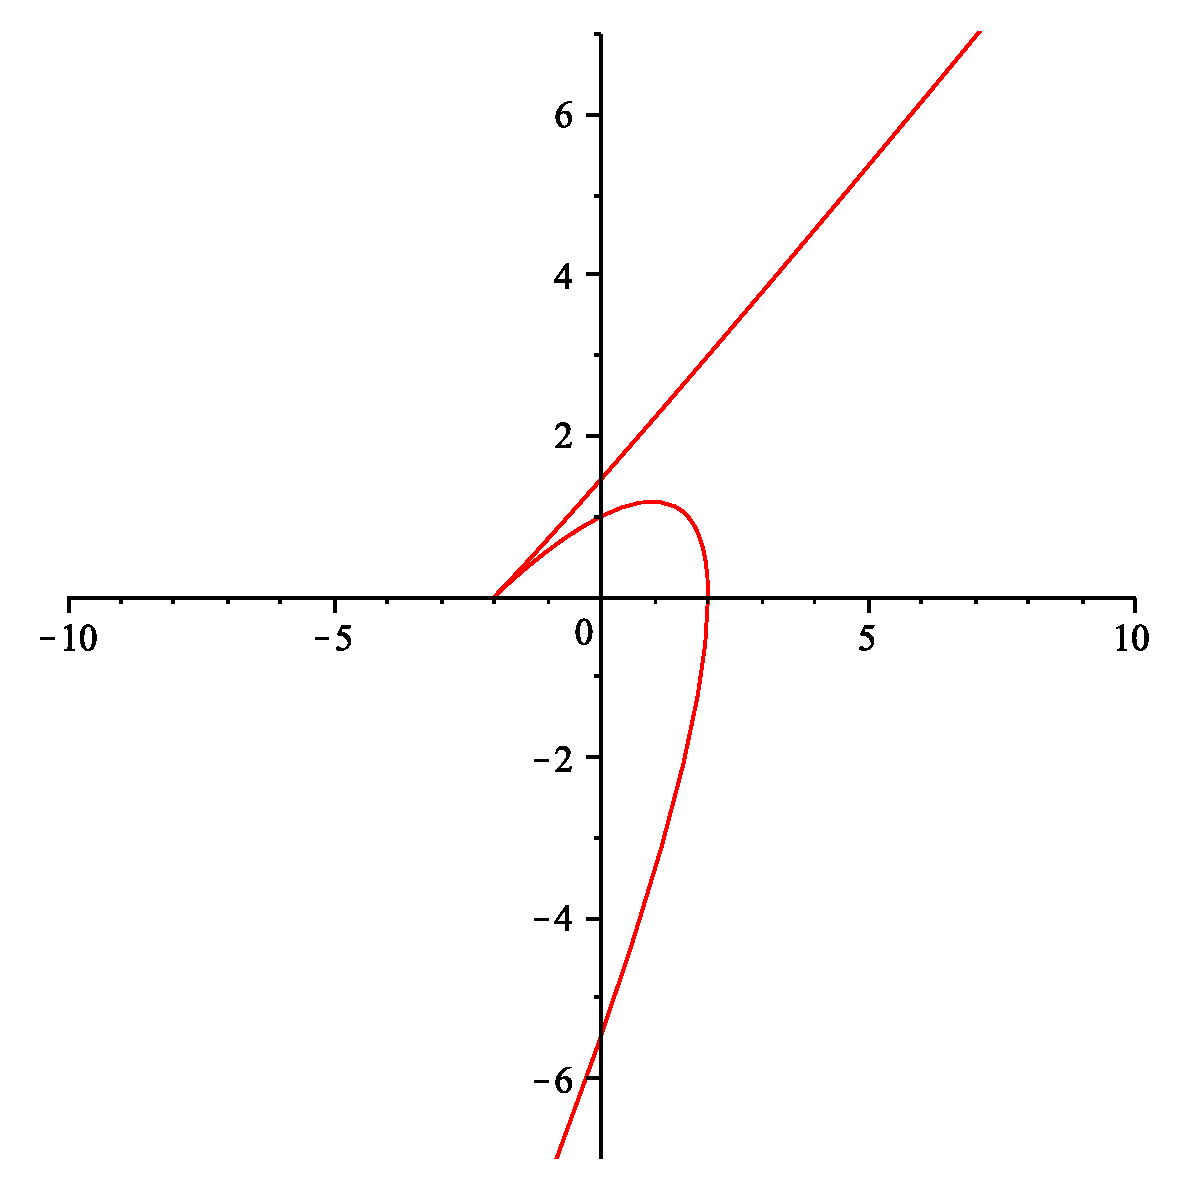
\includegraphics[height=4cm]{../images/img005008-2}}
$$
branche parabolique de coefficient 1}
    \item \question{$x=\sin t$, $y=\dfrac{\cos^2t}{2-\cos t}$           

% %-----------------------------------------------------------------------------
% \vtop to 7cm{\mapleplot{% img27
% x:=sin(t);
% y:=cos(t)^2/(2-cos(t));
% print(plot([x,y,t=0..2*Pi],scaling=constrained));} \par
% \vss}}
\reponse{$$
\centerline{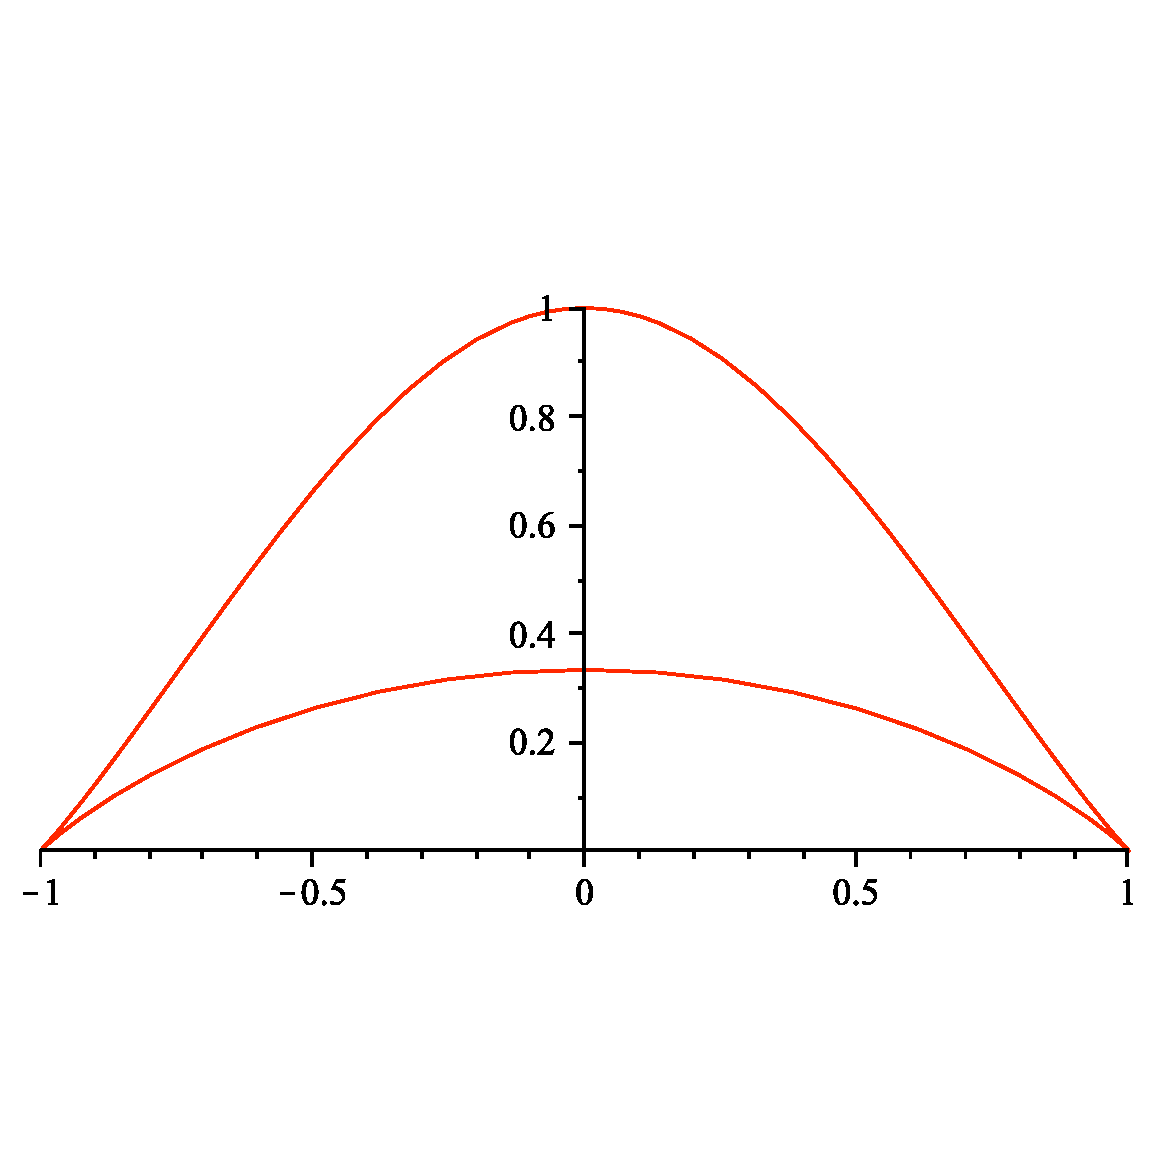
\includegraphics[height=4cm]{../images/img005008-3}}
$$
inflexion : $\cos t = \frac 23$}
    \item \question{$x=(1+\cos^2t)\sin t$, $y=\sin^2t\cos t$               
% %-----------------------------------------------------------------------------
% \vtop to 7cm{\mapleplot{% img28
% x:=(1+cos(t)^2)*sin(t);
% y:=sin(t)^2*cos(t);
% print(plot([x,y,t=0..2*Pi],scaling=constrained));} \par
% \vss}}
\reponse{$$
\centerline{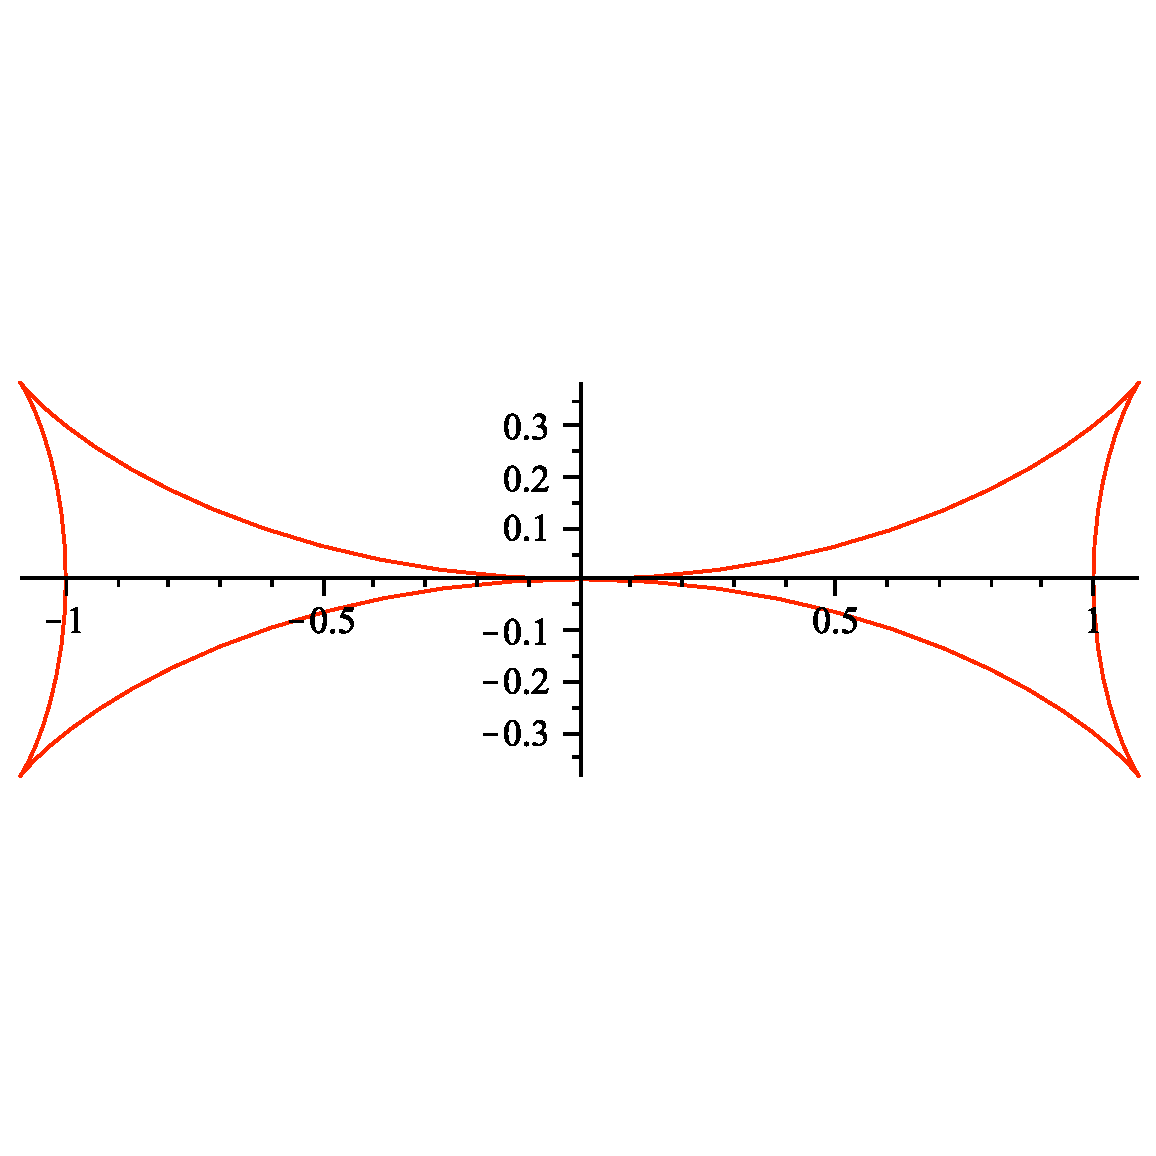
\includegraphics[height=4cm]{../images/img005008-4}}
$$
rebroussement : $\cos^2t=\frac13$.}
    \item \question{$x=(1+\cos t)\sin 2t$, $y=\cos 2t$

% %-----------------------------------------------------------------------------
% \vtop to 7cm{\mapleplot{% img29
% x:=(1+cos(t))*sin(2*t);
% y:=cos(2*t);
% print(plot([x,y,t=0..2*Pi],scaling=constrained));} \par
% \vss}
% 
%}
\reponse{$$
\centerline{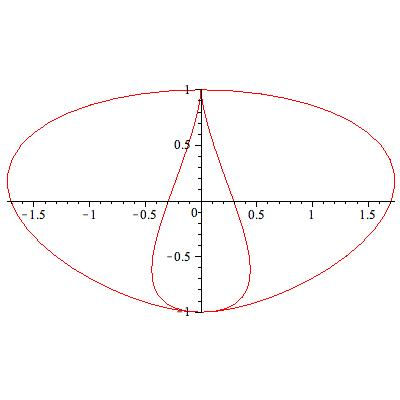
\includegraphics[height=4cm]{../images/img005008-5}}
$$}
\end{enumerate}
}
